%!TEX root = ../egpaper_final.tex

\section{Results}

\subsection{Testing with Other Obstacles}

To demonstrate the robustness of our algorithm, we test it on another set of stairs with a smooth texture and a different number of steps. Despite these differences, we still obtain a reasonable polytope model of the stairs using our algorithm with the Orientation Method (See Section \ref{orient-method}) and the exact same parameters that we used to build the polytope in Figure \ref{polytope-diagonal-orient}. Results could likely be improved by dynamically choosing parameters such as the number of horizontal and vertical planes, the reference normal tolerance, and the number of MSAC iterations online.

\begin{figure}[!h]
\centering
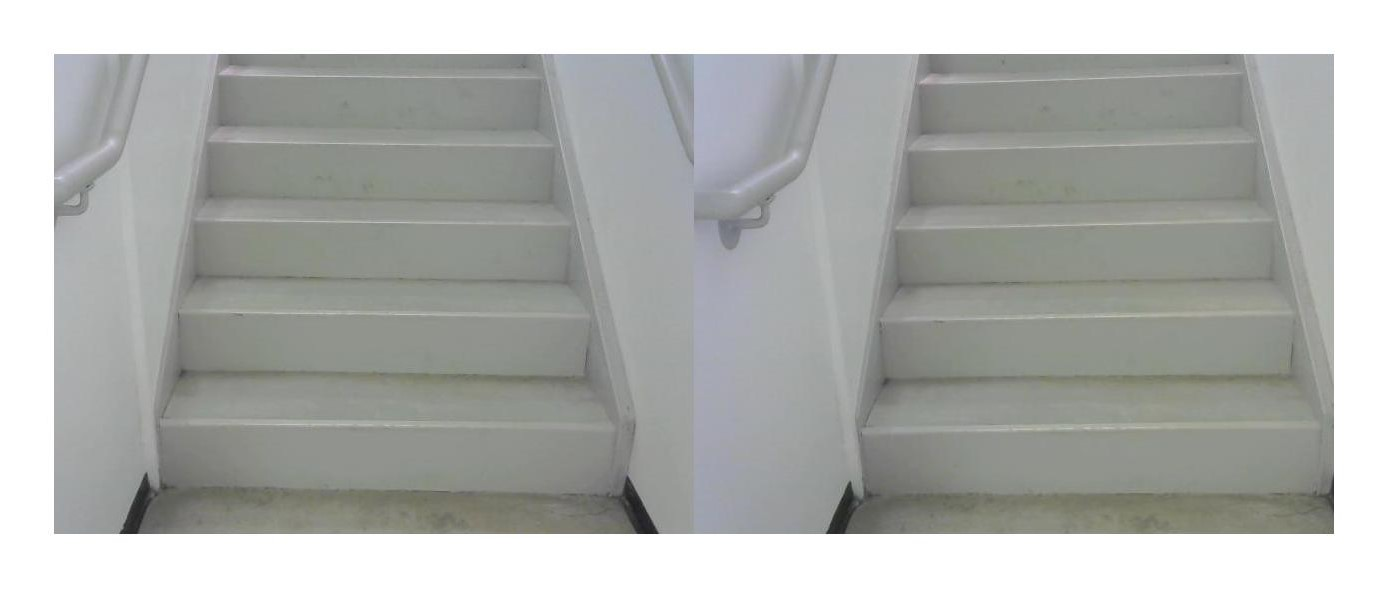
\includegraphics[width=\columnwidth]{Sections/Figures/simmons-stereo-pair.jpg}
\caption{A set of stairs from Simmons Hall. Notice that these stairs have a smooth texture compared to the stairs from Figure \ref{stereo-image-pair}.}
\label{simmons-pair}
\end{figure}

\begin{figure}[!h]
\centering
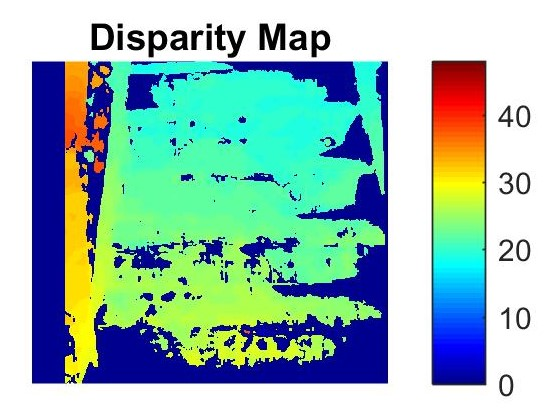
\includegraphics[width=\columnwidth]{Sections/Figures/simmons-stairs-depthmap.jpg}
\caption{The depthmap of the stairs in Figure \ref{simmons-pair}. Despite considerable noise in this depthmap due to a lack of texture on the stairs, our algorithm manages to construct a polytope.}
\label{simmons-depthmap}
\end{figure}

\begin{figure}[!h]
\centering
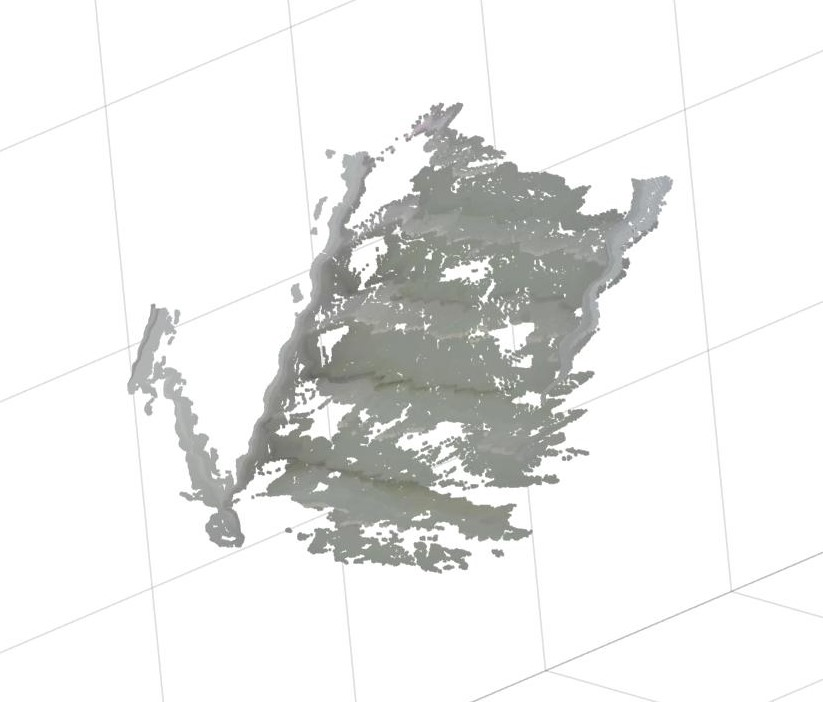
\includegraphics[width=\columnwidth]{Sections/Figures/simmons-stairs-ptcloud.jpg}
\caption{A pointcloud of the Simmons stairs.}
\label{simmons-ptcloud}
\end{figure}

\begin{figure}[!h]
\centering
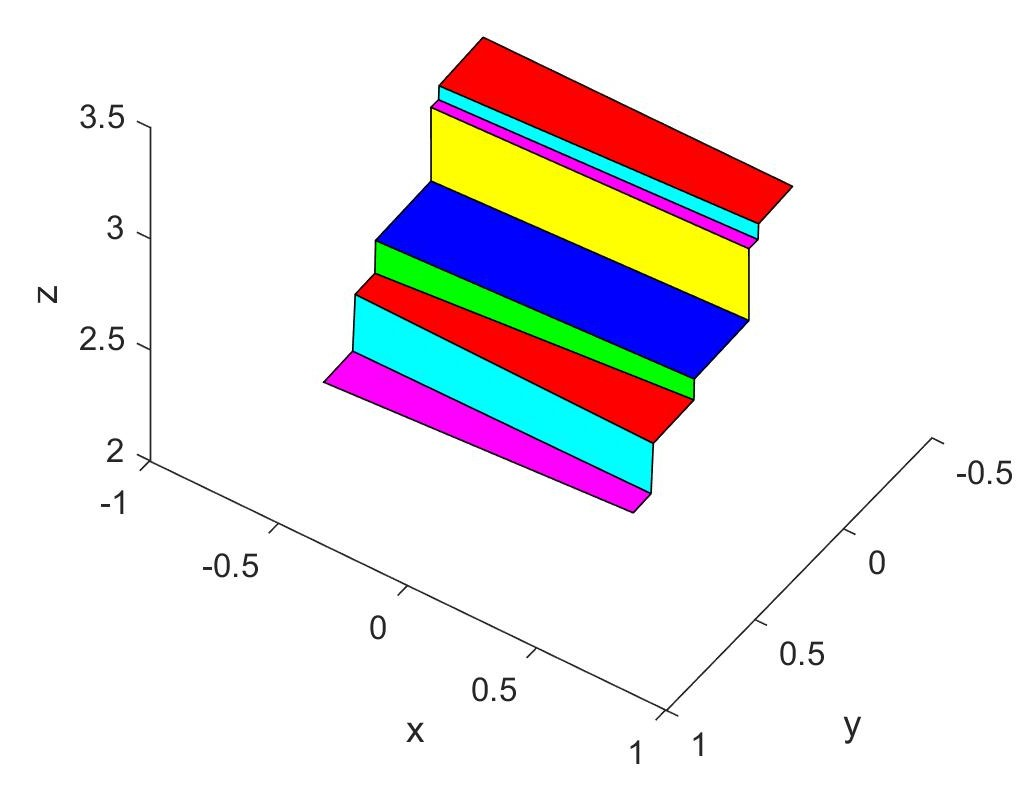
\includegraphics[width=\columnwidth]{Sections/Figures/simmons-stairs-diagonal-geom.jpg}
\caption{The final polytope reconstruction of the Simmons stairs. }
\label{simmons-polytope}
\end{figure}

\subsection{Testing with the Cheetah 3}

Since the robot previously used only reactive sensing of the environment this meant that the only way for the robot to sense obstacles and terrain was to physically interact with them. A robust reactive controller has been achieved and allows the robot to traverse highly unstructured terrains while remaining stable. However, while this makes the robot robust, there are situations where the terrain is not traversable easily without prior knowledge of the environment. Adding the vision system to the overall control system as an input to the path planning as seen in Figure \ref{fig:BD} will allow the robot to know if an obstacle is present, where it is, and its dimensions. Then it can decide how to modify its locomotion plan accordingly. For purposes of this demo the robot will attempt to detect the stair height and distance and modify its swing leg trajectory to place it on the stairs as its nominal swing foot height is lower than an average step.
\begin{figure}[!h]
\centering
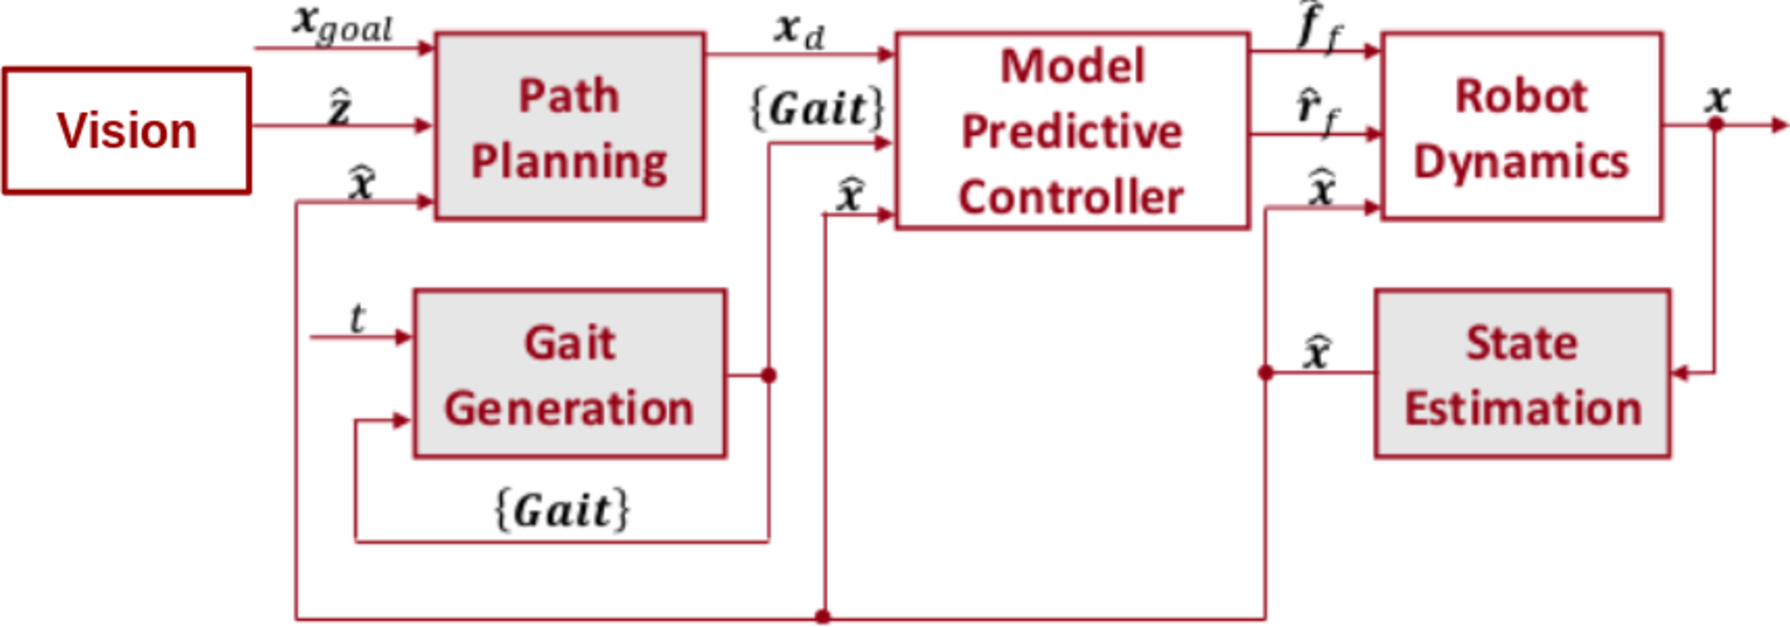
\includegraphics[width=\columnwidth]{Figures/BlockDiagram.pdf}
\caption{.}
\label{fig:BD}
\end{figure}

It is not enough to just find the dimensions of the object in front of the robot. This doesn't have any physical meaning to the robot until we find the relationship between the reconstructed object to the robot's coordinate frame. We take the points of interest of the object in the 3D camera frame, ${}^\mathcal{C}\bm{p}_o$, and apply the following transformation

\begin{equation}
{}^\mathcal{I}\bm{p}_o = {}^\mathcal{I}\bm{H}_\mathcal{C}{}^\mathcal{C}\bm{p}_o
\end{equation}

where ${}^\mathcal{I}\bm{H}_\mathcal{C}$ is the homogeneous transformation matrix between the camera frame and the Inertial frame. This allows the robot to know the distance and angle to the stairs relative to its body as seen in Figure \ref{fig:RSR}. With this, the robot now has knowledge about its environment without the need to physically interact with it. 
\begin{figure}[!h]
\centering
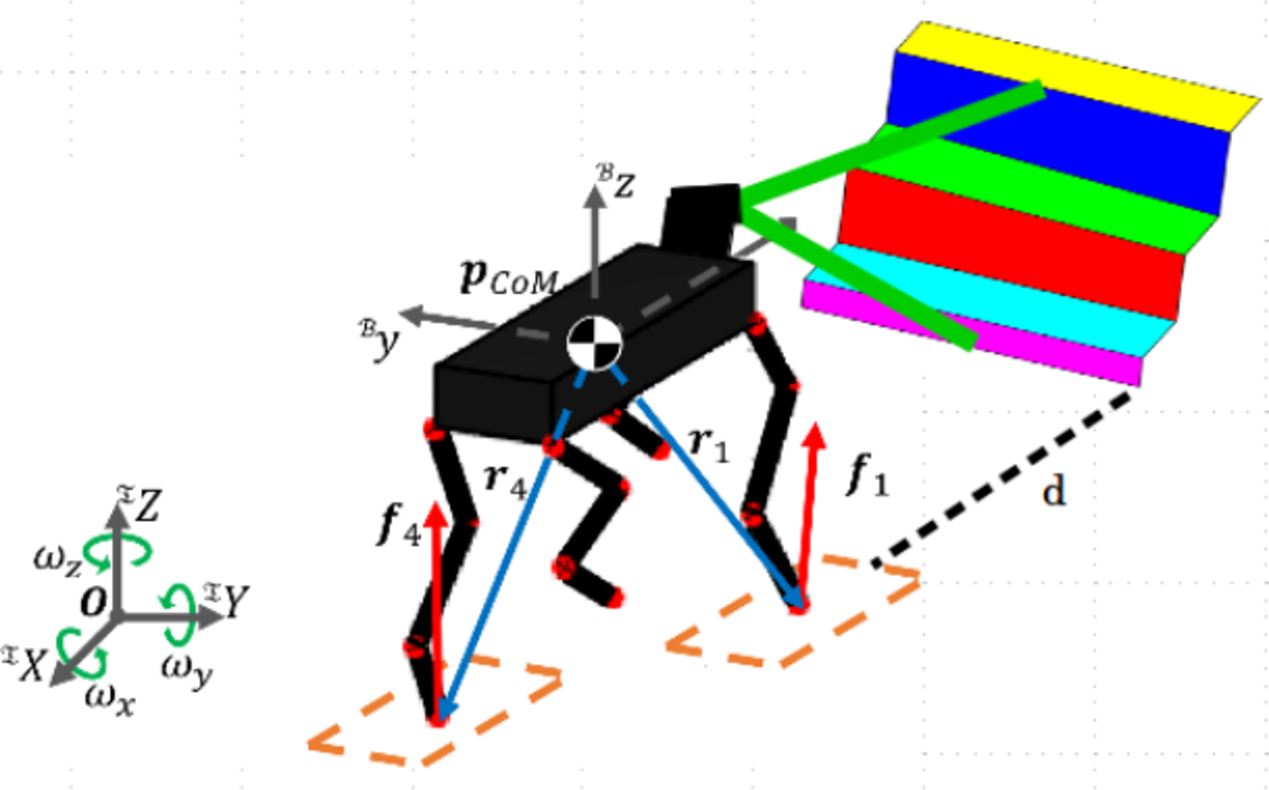
\includegraphics[width=\columnwidth]{Figures/RobotStairsRelation.pdf}
\caption{The robot must transform the coordinates of the stairs in the 3D reconstructed camera frame into the world frame in relation to the robot.}
\label{fig:RSR}
\end{figure}
With the robot holding an internal model of the environment with respect to its state, the path planner can adapt the nominal gait and foot placement trajectory to deal with the stairs at the detected height. The foot trajectory is modified when the robot's center of mass has traveled close enough to the detected stairs
\begin{equation}
({}^\Psi\bm{p}_{CoM,x} - {}^\Psi\bm{p}_{0,x}) < (d - d_{buffer})
\end{equation}
where ${}^\Psi\bm{p}_{CoM,x}$ is the yaw rotated CoM position ignoring pitch and roll effects, ${}^\Psi\bm{p}_{0,x}$ is the yaw rotated position at the last vision input, $d$ is the distance to the object at the detection time, and $d_{buffer}$ is a user defined buffer distance so that the robot begins lifting the legs slightly before the actual stair.


The vision system was successfully integrated with the robot software pipeline. Testing was first done in simulation where the webcams were used to detect the stairs and the robot was walked forward in simulation. The nominal trotting swing height for the leg trajectories is about 15 cm and the stair height was 21 cm. Therefore, the path planner made the decision to raise the height of the trajectory to about 30 cm, which was approximately 10 cm over the detected object height. When it reached the location of the 3D reconstructed stairs, the robot modified its foot trajectory appropriately. 

The pair of cameras was mounted on the physical robot and experiments were run with the real stair set on a treadmill. Figure \ref{fig:RS} shows the robot successfully climbing the stairs on its first attempt. With the terrain-blind controller, the most common failure mode was the robot being unable to get its leg over the stair and tripping. With the vision input, this was no longer the case as it knew how high to lift its leg and where to place the feet to aquire an adequate foothold.
\begin{figure}[!h]
\centering
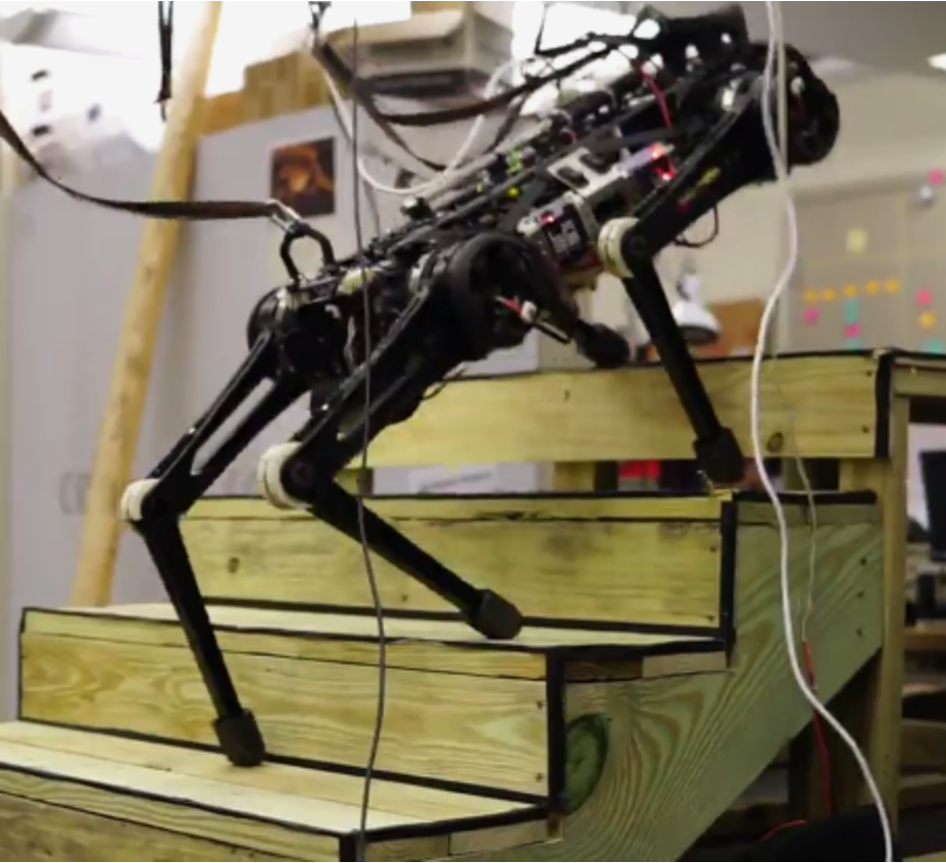
\includegraphics[width=0.85\columnwidth]{Figures/RobotStairs.pdf}
\caption{With the vision input, the robot is able to stably figure out how high to raise the feet in order to place them onto the stairs and successfully climb up.}
\label{fig:RS}
\end{figure}